% Options for packages loaded elsewhere
\PassOptionsToPackage{unicode}{hyperref}
\PassOptionsToPackage{hyphens}{url}
\PassOptionsToPackage{dvipsnames,svgnames,x11names}{xcolor}
%
\documentclass[
  letterpaper,
  DIV=11,
  numbers=noendperiod]{scrreprt}

\usepackage{amsmath,amssymb}
\usepackage{iftex}
\ifPDFTeX
  \usepackage[T1]{fontenc}
  \usepackage[utf8]{inputenc}
  \usepackage{textcomp} % provide euro and other symbols
\else % if luatex or xetex
  \usepackage{unicode-math}
  \defaultfontfeatures{Scale=MatchLowercase}
  \defaultfontfeatures[\rmfamily]{Ligatures=TeX,Scale=1}
\fi
\usepackage{lmodern}
\ifPDFTeX\else  
    % xetex/luatex font selection
  \setmainfont[]{DejaVu Sans}
  \setmonofont[Scale=0.75]{Fira Code}
\fi
% Use upquote if available, for straight quotes in verbatim environments
\IfFileExists{upquote.sty}{\usepackage{upquote}}{}
\IfFileExists{microtype.sty}{% use microtype if available
  \usepackage[]{microtype}
  \UseMicrotypeSet[protrusion]{basicmath} % disable protrusion for tt fonts
}{}
\makeatletter
\@ifundefined{KOMAClassName}{% if non-KOMA class
  \IfFileExists{parskip.sty}{%
    \usepackage{parskip}
  }{% else
    \setlength{\parindent}{0pt}
    \setlength{\parskip}{6pt plus 2pt minus 1pt}}
}{% if KOMA class
  \KOMAoptions{parskip=half}}
\makeatother
\usepackage{xcolor}
\setlength{\emergencystretch}{3em} % prevent overfull lines
\setcounter{secnumdepth}{5}
% Make \paragraph and \subparagraph free-standing
\ifx\paragraph\undefined\else
  \let\oldparagraph\paragraph
  \renewcommand{\paragraph}[1]{\oldparagraph{#1}\mbox{}}
\fi
\ifx\subparagraph\undefined\else
  \let\oldsubparagraph\subparagraph
  \renewcommand{\subparagraph}[1]{\oldsubparagraph{#1}\mbox{}}
\fi

\usepackage{color}
\usepackage{fancyvrb}
\newcommand{\VerbBar}{|}
\newcommand{\VERB}{\Verb[commandchars=\\\{\}]}
\DefineVerbatimEnvironment{Highlighting}{Verbatim}{commandchars=\\\{\}}
% Add ',fontsize=\small' for more characters per line
\usepackage{framed}
\definecolor{shadecolor}{RGB}{241,243,245}
\newenvironment{Shaded}{\begin{snugshade}}{\end{snugshade}}
\newcommand{\AlertTok}[1]{\textcolor[rgb]{0.68,0.00,0.00}{#1}}
\newcommand{\AnnotationTok}[1]{\textcolor[rgb]{0.37,0.37,0.37}{#1}}
\newcommand{\AttributeTok}[1]{\textcolor[rgb]{0.40,0.45,0.13}{#1}}
\newcommand{\BaseNTok}[1]{\textcolor[rgb]{0.68,0.00,0.00}{#1}}
\newcommand{\BuiltInTok}[1]{\textcolor[rgb]{0.00,0.23,0.31}{#1}}
\newcommand{\CharTok}[1]{\textcolor[rgb]{0.13,0.47,0.30}{#1}}
\newcommand{\CommentTok}[1]{\textcolor[rgb]{0.37,0.37,0.37}{#1}}
\newcommand{\CommentVarTok}[1]{\textcolor[rgb]{0.37,0.37,0.37}{\textit{#1}}}
\newcommand{\ConstantTok}[1]{\textcolor[rgb]{0.56,0.35,0.01}{#1}}
\newcommand{\ControlFlowTok}[1]{\textcolor[rgb]{0.00,0.23,0.31}{#1}}
\newcommand{\DataTypeTok}[1]{\textcolor[rgb]{0.68,0.00,0.00}{#1}}
\newcommand{\DecValTok}[1]{\textcolor[rgb]{0.68,0.00,0.00}{#1}}
\newcommand{\DocumentationTok}[1]{\textcolor[rgb]{0.37,0.37,0.37}{\textit{#1}}}
\newcommand{\ErrorTok}[1]{\textcolor[rgb]{0.68,0.00,0.00}{#1}}
\newcommand{\ExtensionTok}[1]{\textcolor[rgb]{0.00,0.23,0.31}{#1}}
\newcommand{\FloatTok}[1]{\textcolor[rgb]{0.68,0.00,0.00}{#1}}
\newcommand{\FunctionTok}[1]{\textcolor[rgb]{0.28,0.35,0.67}{#1}}
\newcommand{\ImportTok}[1]{\textcolor[rgb]{0.00,0.46,0.62}{#1}}
\newcommand{\InformationTok}[1]{\textcolor[rgb]{0.37,0.37,0.37}{#1}}
\newcommand{\KeywordTok}[1]{\textcolor[rgb]{0.00,0.23,0.31}{#1}}
\newcommand{\NormalTok}[1]{\textcolor[rgb]{0.00,0.23,0.31}{#1}}
\newcommand{\OperatorTok}[1]{\textcolor[rgb]{0.37,0.37,0.37}{#1}}
\newcommand{\OtherTok}[1]{\textcolor[rgb]{0.00,0.23,0.31}{#1}}
\newcommand{\PreprocessorTok}[1]{\textcolor[rgb]{0.68,0.00,0.00}{#1}}
\newcommand{\RegionMarkerTok}[1]{\textcolor[rgb]{0.00,0.23,0.31}{#1}}
\newcommand{\SpecialCharTok}[1]{\textcolor[rgb]{0.37,0.37,0.37}{#1}}
\newcommand{\SpecialStringTok}[1]{\textcolor[rgb]{0.13,0.47,0.30}{#1}}
\newcommand{\StringTok}[1]{\textcolor[rgb]{0.13,0.47,0.30}{#1}}
\newcommand{\VariableTok}[1]{\textcolor[rgb]{0.07,0.07,0.07}{#1}}
\newcommand{\VerbatimStringTok}[1]{\textcolor[rgb]{0.13,0.47,0.30}{#1}}
\newcommand{\WarningTok}[1]{\textcolor[rgb]{0.37,0.37,0.37}{\textit{#1}}}

\providecommand{\tightlist}{%
  \setlength{\itemsep}{0pt}\setlength{\parskip}{0pt}}\usepackage{longtable,booktabs,array}
\usepackage{calc} % for calculating minipage widths
% Correct order of tables after \paragraph or \subparagraph
\usepackage{etoolbox}
\makeatletter
\patchcmd\longtable{\par}{\if@noskipsec\mbox{}\fi\par}{}{}
\makeatother
% Allow footnotes in longtable head/foot
\IfFileExists{footnotehyper.sty}{\usepackage{footnotehyper}}{\usepackage{footnote}}
\makesavenoteenv{longtable}
\usepackage{graphicx}
\makeatletter
\def\maxwidth{\ifdim\Gin@nat@width>\linewidth\linewidth\else\Gin@nat@width\fi}
\def\maxheight{\ifdim\Gin@nat@height>\textheight\textheight\else\Gin@nat@height\fi}
\makeatother
% Scale images if necessary, so that they will not overflow the page
% margins by default, and it is still possible to overwrite the defaults
% using explicit options in \includegraphics[width, height, ...]{}
\setkeys{Gin}{width=\maxwidth,height=\maxheight,keepaspectratio}
% Set default figure placement to htbp
\makeatletter
\def\fps@figure{htbp}
\makeatother
\newlength{\cslhangindent}
\setlength{\cslhangindent}{1.5em}
\newlength{\csllabelwidth}
\setlength{\csllabelwidth}{3em}
\newlength{\cslentryspacingunit} % times entry-spacing
\setlength{\cslentryspacingunit}{\parskip}
\newenvironment{CSLReferences}[2] % #1 hanging-ident, #2 entry spacing
 {% don't indent paragraphs
  \setlength{\parindent}{0pt}
  % turn on hanging indent if param 1 is 1
  \ifodd #1
  \let\oldpar\par
  \def\par{\hangindent=\cslhangindent\oldpar}
  \fi
  % set entry spacing
  \setlength{\parskip}{#2\cslentryspacingunit}
 }%
 {}
\usepackage{calc}
\newcommand{\CSLBlock}[1]{#1\hfill\break}
\newcommand{\CSLLeftMargin}[1]{\parbox[t]{\csllabelwidth}{#1}}
\newcommand{\CSLRightInline}[1]{\parbox[t]{\linewidth - \csllabelwidth}{#1}\break}
\newcommand{\CSLIndent}[1]{\hspace{\cslhangindent}#1}

\KOMAoption{captions}{tableheading}
\makeatletter
\makeatother
\makeatletter
\@ifpackageloaded{bookmark}{}{\usepackage{bookmark}}
\makeatother
\makeatletter
\@ifpackageloaded{caption}{}{\usepackage{caption}}
\AtBeginDocument{%
\ifdefined\contentsname
  \renewcommand*\contentsname{Table of contents}
\else
  \newcommand\contentsname{Table of contents}
\fi
\ifdefined\listfigurename
  \renewcommand*\listfigurename{List of Figures}
\else
  \newcommand\listfigurename{List of Figures}
\fi
\ifdefined\listtablename
  \renewcommand*\listtablename{List of Tables}
\else
  \newcommand\listtablename{List of Tables}
\fi
\ifdefined\figurename
  \renewcommand*\figurename{Figure}
\else
  \newcommand\figurename{Figure}
\fi
\ifdefined\tablename
  \renewcommand*\tablename{Table}
\else
  \newcommand\tablename{Table}
\fi
}
\@ifpackageloaded{float}{}{\usepackage{float}}
\floatstyle{ruled}
\@ifundefined{c@chapter}{\newfloat{codelisting}{h}{lop}}{\newfloat{codelisting}{h}{lop}[chapter]}
\floatname{codelisting}{Listing}
\newcommand*\listoflistings{\listof{codelisting}{List of Listings}}
\makeatother
\makeatletter
\@ifpackageloaded{caption}{}{\usepackage{caption}}
\@ifpackageloaded{subcaption}{}{\usepackage{subcaption}}
\makeatother
\makeatletter
\@ifpackageloaded{tcolorbox}{}{\usepackage[skins,breakable]{tcolorbox}}
\makeatother
\makeatletter
\@ifundefined{shadecolor}{\definecolor{shadecolor}{rgb}{.97, .97, .97}}
\makeatother
\makeatletter
\makeatother
\makeatletter
\makeatother
\ifLuaTeX
\usepackage[bidi=basic]{babel}
\else
\usepackage[bidi=default]{babel}
\fi
\babelprovide[main,import]{english}
% get rid of language-specific shorthands (see #6817):
\let\LanguageShortHands\languageshorthands
\def\languageshorthands#1{}
\ifLuaTeX
  \usepackage{selnolig}  % disable illegal ligatures
\fi
\IfFileExists{bookmark.sty}{\usepackage{bookmark}}{\usepackage{hyperref}}
\IfFileExists{xurl.sty}{\usepackage{xurl}}{} % add URL line breaks if available
\urlstyle{same} % disable monospaced font for URLs
\hypersetup{
  pdftitle={Production of seasonally adjusted series},
  pdfauthor={Anna Smyk; Tanguy Barthelemy},
  pdflang={en},
  colorlinks=true,
  linkcolor={blue},
  filecolor={Maroon},
  citecolor={Blue},
  urlcolor={Blue},
  pdfcreator={LaTeX via pandoc}}

\title{Production of seasonally adjusted series}
\author{Anna Smyk \and Tanguy Barthelemy}
\date{2026-04-02}

\begin{document}
\maketitle
\ifdefined\Shaded\renewenvironment{Shaded}{\begin{tcolorbox}[sharp corners, enhanced, frame hidden, boxrule=0pt, interior hidden, borderline west={3pt}{0pt}{shadecolor}, breakable]}{\end{tcolorbox}}\fi

\renewcommand*\contentsname{Table of contents}
{
\hypersetup{linkcolor=}
\setcounter{tocdepth}{2}
\tableofcontents
}
\bookmarksetup{startatroot}

\hypertarget{ind}{%
\chapter*{JDemetra+ and R Cookbook}\label{ind}}
\addcontentsline{toc}{chapter}{JDemetra+ and R Cookbook}

\markboth{JDemetra+ and R Cookbook}{JDemetra+ and R Cookbook}

Seasonal adjustment is a key process in official statistics, as it is
necessary for the dissemination and interpretation of a large number of
economic indicators. In an effort to harmonize practices, Eurostat has
recommended since 2015 the use of the open source software JDemetra+,
which provides access to the two most popular seasonal adjustment
algorithms in European statistical agencies: X-13 Arima and Tramo-Seats,
via a graphical user interface and a family of R packages.

These pages describe and illustrate how to take advantage of JDemetra+
version 3 to build efficient production processes that can adjust
several thousand series with individualized settings, while controlling
statistical quality and minimizing manual fine-tuning.

\bookmarksetup{startatroot}

\hypertarget{introduction}{%
\chapter*{Introduction}\label{introduction}}
\addcontentsline{toc}{chapter}{Introduction}

\markboth{Introduction}{Introduction}

Seasonal adjustment is a key process in official statistics. The
dissemination of most economic indicators requires that they first be
purged of quasi-periodic, seasonal, and calendar movements in order to
facilitate the interpretation of short-term developments and the
identification of turning points and medium- and long-term trends (Bell
and Hillmer 1984). However, implementing a standardized and flexible
process for producing seasonally and calendar adjusted (sa) series that
complies with European statistical system best practices (Eurostat 2024)
is costly. In addition to producing seasonally adjusted series, it must
also provide integrated quality indicators (Kirchner and alli 2018) and
allow for manual adjustment by experts, often under significant time
constraints. At INSEE, all seasonal adjustment processes are based on
JDemetra+ (Smyk and alli 2026), officially recommended by Eurostat since
2015. This open source software for time series analysis provides access
to the two most popular seasonal adjustment algorithms in European
official statistics: X-13 Arima (US-Census-Bureau 2015) and Tramo-Seats
(Gomez and Maravall 1996). The algorithms are written in Java and
accessible via a \href{https://github.com/jdemetra}{Graphical User
Interface~🔗} and a family of R packages: the
\href{https://github.com/rjdverse}{rjdverse~🔗}.

Version 3 of JDemetra+, available since 2023, offers new R tools to
improve production processes. In addition, the Covid crisis has
highlighted the need for fine-grained parameterization on a very large
scale, such as assigning specific outlier profiles to each series for
several hundred series. Finally, the emphasis in recent years on the
transition from SAS to R at INSEE is promoting the acceptance of these
new tools in a general context of modernization. Therefore, the current
context is very favorable for reviewing and optimizing existing
processes.

Each year, INSEE's Statistical Methods Department undertakes a number of
process redesigns, disseminates best practices, and trains producers in
the use of the JDemetra+ software. However, in order to clarify the
construction and optimization of seasonality adjustment processes, an
example of a method and a presentation of the latest tools are
necessary.

Currently, producers of seasonally adjusted series have access to
theoretical information on seasonal adjustment algorithms, such as the
\href{https://ec.europa.eu/eurostat/web/products-manuals-and-guidelines/-/ks-gq\%20-18-001}{Handbook
on Seasonal Adjustment~🔗}, a guide to
\href{https://ec.europa.eu/eurostat/web/products-manuals-and-guidelines/w/ks-gq\%20-24-012}{best
practices~🔗}, the \href{https://doc.jdemetra.org/}{JDemetra+ software
documentation~🔗}, and possibly notes reflecting the historical
sedimentation of practices in your institution. One piece seems to be
missing from this puzzle: a specific example of implementation using the
most up-to-date tools. The rest of this article aims to describe and
illustrate how to take advantage of JDemetra+ version 3.x to build
efficient production processes, adjust up to several thousand series
with individualized settings, control statistical quality, and target
manual fine-tuning.

The production of seasonally adjusted series generally involves three
stages: the process of installation, during which methodological changes
are most significant; annual revision campaigns; and infra-annual
revision campaigns. Production processes can be based on
\emph{workspaces}---a data structure specific to JDemetra+ that allows
for the use of a graphical interface---or be built entirely in R.

Annual campaigns require tools for comparing and prioritizing models in
need of manual fine-tuning. The R package JDCruncheR can be used for
this purpose. Infra-annual production requires data revision policies
and tools for analysis of revisions to validate figures before
publication. We detail these three phases by showing the advantages and
disadvantages of different configurations, presenting available tools,
and comparing execution times. The article includes R code snippets, and
a complete example is available in the
\href{https://inseefr.github.io/rjd3production/articles/process.html}{\{rjd3production\}
package~🔗}

Following a brief overview of the statistical operations comprising the
seasonal adjustment process and the JDemetra+ software, the second
section outlines the construction of a production process. The third
section covers annual and infra-annual reviews of parameters. The
appendices provide a more detailed presentation of the reviewed tools.

\bookmarksetup{startatroot}

\hypertarget{part-1-seasonal-adjustment-and-production}{%
\chapter*{Part 1: Seasonal Adjustment and
Production}\label{part-1-seasonal-adjustment-and-production}}
\addcontentsline{toc}{chapter}{Part 1: Seasonal Adjustment and
Production}

\markboth{Part 1: Seasonal Adjustment and Production}{Part 1: Seasonal
Adjustment and Production}

\hypertarget{the-statistical-process}{%
\section*{The statistical process}\label{the-statistical-process}}
\addcontentsline{toc}{section}{The statistical process}

\markright{The statistical process}

Seasonal adjustment removes periodic movements from the data series that
mask cyclical variations and long-term trends. For this reason, most
economic indicators are published seasonally (and calendar) adjusted
(SA). Seasonal adjustment requires estimating a seasonal component that
captures all periodic intra-annual movements in order to remove it from
the raw series \(Y_\text{CVS} = Y-S\). To do this, the raw series is
broken down into three unobservable components: seasonality, trend, and
irregularity (\(Y=S+T+I\)), where the trend \(T\) represents long-term
movements and \(I\) represents noise generated by exceptional events
(strikes, weather conditions, short-term shocks, etc.) and all
measurement errors. The algorithms most commonly used today by European
national statistical institutes and central banks are Tramo-Seats (Gomez
and Maravall 1996) and X13-Arima (US-Census-Bureau 2015). These methods
proceed in two stages: the raw series is not directly decomposed but
first linearized, by (permanently) removing calendar effects and
(temporarily) removing outliers using Reg-Arima modelling.

\hypertarget{objectives}{%
\subsection*{Objectives}\label{objectives}}
\addcontentsline{toc}{subsection}{Objectives}

The main objective is, of course, to produce seasonally adjusted (SA)
series, particularly with a view to publication. However, to ensure the
quality of the seasonal adjustment, a broader output is necessary. The
process must therefore allow the diagnostics to be viewed (seasonality
tests, residual seasonality tests, and residual calendar effects for the
seasonally adjusted series, etc.) and the parameters to be adjusted in
light of the problems identified by these diagnostics. Intermediate
series, in addition to the final SA series, such as unobservable
components, the linearized series, and seasonal factors (including
forecast factors), are often useful.

\hypertarget{steps}{%
\subsection*{Steps}\label{steps}}
\addcontentsline{toc}{subsection}{Steps}

Seasonal adjustment begins with a seasonality test to ensure that this
operation is necessary for the series in question. If this is not the
case, the raw series will also be published as SA. In practice, this
test is often performed at the end of the seasonal adjustment process,
which allows it to be performed on the linearized series (from which the
\(S\) factors will be extracted) and to always keep the same input data
set, excluding only the series that are not to be seasonally adjusted at
the dissemination stage.

A correction for calendar effects must often be implemented or at least
tested
\footnote{Eurostat guidelines recommend to correct calendar effects that have ex-ante relevance.}.
The first estimation (pre-adjustment and decomposition) can then be
made, probably with a largely automatic specification, and a quality
report can be generated to improve the quality of the seasonal
adjustment. We refer here to a quality report and not simply to
diagnostics, as the former consists of formatting the diagnostics and
summarizing them in a score that allows a \emph{selective editing}
approach to prioritize manual fine-tuning in the series. It is generally
necessary to quantify the revisions and the numerical impact of the
choice of parameters, which will influence the choice of final
parameters. Once these elements have been reviewed, a second estimation
can be made, and the process may be repeated until a final set of
parameters is reached.

Table 1: The steps

\begin{longtable}[]{@{}
  >{\raggedright\arraybackslash}p{(\columnwidth - 2\tabcolsep) * \real{0.4444}}
  >{\raggedright\arraybackslash}p{(\columnwidth - 2\tabcolsep) * \real{0.5556}}@{}}
\toprule\noalign{}
\begin{minipage}[b]{\linewidth}\raggedright
Domain
\end{minipage} & \begin{minipage}[b]{\linewidth}\raggedright
Operations
\end{minipage} \\
\midrule\noalign{}
\endhead
\bottomrule\noalign{}
\endlastfoot
Correction of calendar effects & Creation of a reference calendar \\
& Generation of regression sets \\
& Selection of the best set for each series \\
Customization of specifications & Assignment of calendar regressors \\
& Assigning outliers \\
& Other parameters \\
Estimation & Preliminary estimation \\
& Output generation \\
Quality Control & Quality Report \\
& Manual fine tuning \\
& Final estimation \\
& Final output generation \\
\end{longtable}

\hypertarget{the-production-process}{%
\section*{The production process}\label{the-production-process}}
\addcontentsline{toc}{section}{The production process}

\markright{The production process}

\hypertarget{properties}{%
\subsection*{Properties}\label{properties}}
\addcontentsline{toc}{subsection}{Properties}

Production inherently requires the automation of as many operations as
possible (definition of specifications, estimation, production of a
quality report, application of revision policies), but also, in the case
of seasonality adjustment, the visualization of diagnostics and graphs
in an environment that allows for rapid manual adjustment of parameters.

The process can be divided into three distinct phases based on their
objectives and the type of intervention they require: implementation of
a production process, annual campaigns, and infra-annual campaigns.

\hypertarget{set-up}{%
\subsection*{Set-up}\label{set-up}}
\addcontentsline{toc}{subsection}{Set-up}

The process must be initialized by making medium-term choices that will
not, in principle, be called into question for a period of approximately
five years. User requirements are then specified: the variables of
interest to be seasonally adjusted are selected, as well as the level of
the nomenclature and the direct (seasonal adjustment at each level) or
indirect (aggregation of seasonally adjusted series) approach. See
Guidelines chapter 5.4 for more details. The relevance of a calendar
effect correction must be tested. This is also the time to determine the
length of the estimation period (\emph{Ibid.}, Chapter 8) and the depth
of revisions during publication (\emph{Ibid.}, Chapter 6). This is also
when the algorithm and software to be used should be chosen.

\hypertarget{annual-and-infra-annual-reviews}{%
\subsection*{Annual and infra-annual
reviews}\label{annual-and-infra-annual-reviews}}
\addcontentsline{toc}{subsection}{Annual and infra-annual reviews}

Approximately once a year, the producer updates the statistical
parameters based on new raw data (\emph{Ibid.}, Chapter 6). One method
is to compare current models with an automatic re-estimation, as
described in Part 3.

During infra-annual production, the goal is to minimize technical
revisions. It is recommended that you review only a limited number of
parameters, and you may even use the seasonal coefficients predicted
during the last annual campaign. The focus should be on revisions and on
the appearance or disappearance of outliers in the recent period.

The rest of this article presents a procedure and the tools needed to
implement the three phases described above. As part of harmonizing
statistical practices and tools, Eurostat has recommended JDemetra+ to
member countries of the European Statistical System for seasonal
adjustment since 2015. We will therefore use this software. The
following section briefly presents its main features relating to the
production of seasonally adjusted series.

\hypertarget{jdemetra-a-tool-for-seasonal-adjustment}{%
\section*{JDemetra+: a tool for seasonal
adjustment}\label{jdemetra-a-tool-for-seasonal-adjustment}}
\addcontentsline{toc}{section}{JDemetra+: a tool for seasonal
adjustment}

\markright{JDemetra+: a tool for seasonal adjustment}

JDemetra+ is an open-source library of algorithms for time series
analysis. These are accessible via a Graphical User Interface (GUI),
which can be enhanced with
\href{https://doc.jdemetra.org/t-plug-ins}{plug-ins~🔗} and an ecosystem
of R packages, the
\href{https://github.com/rjdverse?view_as=public}{rjdverse~🔗}. In
addition to seasonal adjustment, they also enable nowcasting,
benchmarking, temporal disaggregation, trend estimation, and revision
analysis. The development and promotion of JDemetra+ are co-financed by
Eurostat through successive grants and currently within the
\href{https://doc.jdemetra.org/\#COSA-abstract}{COSA~🔗} project.

Seasonal adjustment is the area for which JDemetra+ is best known. The
software was initially developed as a simple graphical interface, based
on the original programs for the two algorithms X12-arima and
Tramo-Seats. The aim was to provide users with a user-friendly view of
the results, diagnostics, and parameters, and to harmonize this for both
algorithms. The software was initially called
\href{https://github.com/cosa-tsa-shop/Resources-Logistics/tree/main/Historical\%20Documents}{Demetra~🔗},
the goddess of agriculture and the seasons. When the Fortran programs of
the US Census Bureau and the Bank of Spain were rewritten in
Java\footnote{Same structure but potentially different estimation and optimization procedures that could give rise to numerically non-strictly equal results.},
Demetra became JDemetra+ (Grudkowska et al. 2013).

\hypertarget{algorithms}{%
\subsection*{Algorithms}\label{algorithms}}
\addcontentsline{toc}{subsection}{Algorithms}

JDemetra+ now offers additional algorithms for seasonal adjustment, but
only the two historical ones are really designed for mass data
production, as they allow parameters to be stored in a \emph{workspace}
and use an automation module called Cruncher. In our examples, we will
refer to X13-Arima, but all recommendations remain valid with
Tramo-Seats.

Table 2: Seasonal adjustment algorithms

\begin{longtable}[]{@{}
  >{\raggedright\arraybackslash}p{(\columnwidth - 6\tabcolsep) * \real{0.3425}}
  >{\raggedright\arraybackslash}p{(\columnwidth - 6\tabcolsep) * \real{0.0685}}
  >{\raggedright\arraybackslash}p{(\columnwidth - 6\tabcolsep) * \real{0.2466}}
  >{\raggedright\arraybackslash}p{(\columnwidth - 6\tabcolsep) * \real{0.3425}}@{}}
\toprule\noalign{}
\begin{minipage}[b]{\linewidth}\raggedright
Algorithm
\end{minipage} & \begin{minipage}[b]{\linewidth}\raggedright
GUI
\end{minipage} & \begin{minipage}[b]{\linewidth}\raggedright
Packages R
\end{minipage} & \begin{minipage}[b]{\linewidth}\raggedright
Suitable for production
\end{minipage} \\
\midrule\noalign{}
\endhead
\bottomrule\noalign{}
\endlastfoot
X13-ARIMA & ✅ & \{rjd3x13\} & yes \\
Tramo-Seats & ✅ & \{rjd3tramoseats\} & yes \\
X12+ & ✅ & \{rjd3x11plus\} & not yet \\
STL & ✅ & \{rjd3stl\} & not yet \\
Basic Structural Models & ✅ & \{rjd3sts\} & not yet \\
\end{longtable}

All of the above algorithms can be used to seasonally adjust monthly,
quarterly, bimonthly, four-monthly, and biannual data. They also have
extensions for high-frequency (infra-monthly) data, as detailed in Webel
and Smyk (2024).

\hypertarget{tools}{%
\subsection*{Tools}\label{tools}}
\addcontentsline{toc}{subsection}{Tools}

\hypertarget{graphical-user-interface-gui}{%
\subsubsection*{Graphical User Interface
(GUI)}\label{graphical-user-interface-gui}}
\addcontentsline{toc}{subsubsection}{Graphical User Interface (GUI)}

JDemetra+ is available as a
\href{https://doc.jdemetra.org/t-gui-overview}{Graphical User
Interface~🔗} designed to facilitate manual fine-tuning through an
organized presentation of results and parameters. Operations are mainly
performed by clicking buttons, which requires auxiliary automation
tools. Using the GUI and the \emph{Cruncher} also requires organizing
data into a specific structure: the
\protect\hyperlink{sec-concept-workspace}{\emph{workspace}~🔗}.

\hypertarget{Cruncher}{%
\subsubsection*{Cruncher}\label{Cruncher}}
\addcontentsline{toc}{subsubsection}{Cruncher}

The \emph{Cruncher} avoids opening the interface and clicking when
launching or refreshing an estimation. It is a command line executable
module that we will use later with two R packages, rjwsacruncher for
estimations and exporting results, and JDCruncher for formatting
diagnostics. Another advantage of the \emph{Cruncher} is its speed: it
can be run on hundreds or thousands of series and produce results in a
reasonable amount of time. The installation procedure and main functions
are described in the
\href{https://doc.jdemetra.org/t-production-tools-Cruncher-qr}{documentation~🔗}.

\hypertarget{r-packages}{%
\subsubsection*{R packages}\label{r-packages}}
\addcontentsline{toc}{subsubsection}{R packages}

A family of packages, \href{https://github.com/rjdverse}{rjdverse~🔗}
provides direct access to JDemetra+ algorithms in R and automates
operations related to the use of \emph{workspaces}. The rjd3production
package offers macro functions corresponding to complete stages in the
production process.

Table 3: R packages for the production of seasonally adjusted series

\begin{longtable}[]{@{}
  >{\raggedright\arraybackslash}p{(\columnwidth - 2\tabcolsep) * \real{0.2917}}
  >{\raggedright\arraybackslash}p{(\columnwidth - 2\tabcolsep) * \real{0.7083}}@{}}
\toprule\noalign{}
\begin{minipage}[b]{\linewidth}\raggedright
Package
\end{minipage} & \begin{minipage}[b]{\linewidth}\raggedright
Useful functions for production
\end{minipage} \\
\midrule\noalign{}
\endhead
\bottomrule\noalign{}
\endlastfoot
\href{https://github.com/rjdverse/rjd3toolkit}{\{rjd3toolkit\}~🔗} &
Generation of calendar regressors, Customization of specifications,
Tests \\
\href{https://github.com/rjdverse/rjd3x13}{\{rjd3x13\}~🔗} & Seasonal
adjustment (Reg-Arima pre-adjustment and X11 decomposition) \\
\href{https://github.com/rjdverse/rjd3tramoseats}{\{rjd3tramoseats\}~🔗}
& Seasonal adjustment (TRAMO pre-adjustment and SEATS decomposition) \\
\href{https://github.com/AQLT/rjwsacruncher}{\{rjwsacruncher\}~🔗} &
\emph{workspace} update and output export \\
\href{https://github.com/InseeFr/JDCruncheR}{\{JDCruncheR\}~🔗} & Create
a quality report for the \emph{workspace} based on the outputs \\
\href{https://github.com/inseefr/rjd3production}{\{rjd3production\}~🔗}
& Wrapper with macro functions for each production step \\
\href{https://github.com/rjdverse/rjd3workspace}{\{rjd3workspace\}~🔗} &
\emph{workspace} creation and modification \\
\href{https://github.com/rjdverse/rjd3providers}{\{rjd3providers\}~🔗} &
Input data management \\
\end{longtable}

The installation procedures for all those tools are to be found in the
\href{https://doc.jdemetra.org/\#installing-the-software}{documentation~🔗}.

\hypertarget{data-structures}{%
\subsection*{Data structures}\label{data-structures}}
\addcontentsline{toc}{subsection}{Data structures}

In the following paragraphs, we briefly describe the data structures and
concepts specific to JDemetra+, which will be useful in the following
sections.

\hypertarget{sec-concept-input}{%
\subsubsection*{Input series}\label{sec-concept-input}}
\addcontentsline{toc}{subsubsection}{Input series}

The JDemetra+ interface accepts different types of data formats that can
be imported from the menus in the
\href{https://doc.jdemetra.org/t-gui-overview\#providers-window}{providers}
tab.

\begin{itemize}
\tightlist
\item
  CSV files (specifying the field separator, date format, decimal
  separator, etc.)
\item
  Excel files (only *.xlsx in version 3.x)
\item
  XML files
\item
  SDMX data sources
\item
  ODBC or JDBC databases
\end{itemize}

All series, whether seasonally adjusted data or auxiliary variables, are
imported in the same way. For estimations, R packages work with TS class
objects.

\hypertarget{sec-concept-output}{%
\subsubsection*{Outputs}\label{sec-concept-output}}
\addcontentsline{toc}{subsubsection}{Outputs}

JDemetra+ generates different types of outputs:

\begin{itemize}
\tightlist
\item
  Series (seasonally adjusted, seasonal factors, linearized series)
\item
  Parameters (specification information)
\item
  Diagnostics (information on the quality of the fit)
\end{itemize}

The graphical interface allows you to view these outputs and export them
using \href{https://doc.jdemetra.org/t-gui-output}{drop-down menus~🔗}.

The \emph{Cruncher} avoids menu navigation by offering an identical
automated export. The parameters and diagnostics are grouped into a
single data file where the identifier is the name of the series. The
exported file is called demetra\_m.CVS, where ``m'' stands for matrix.

If the estimation is done in R, for example with \{rjd3x13\}, a list of
lists groups the series, diagnostics, and parameters.

\begin{Shaded}
\begin{Highlighting}[]
\FunctionTok{library}\NormalTok{(}\StringTok{"rjd3x13"}\NormalTok{)}
\NormalTok{mod }\OtherTok{\textless{}{-}} \FunctionTok{x13}\NormalTok{(my\_series)}
\NormalTok{mod}\SpecialCharTok{$}\NormalTok{result}\SpecialCharTok{$}\NormalTok{final}
\end{Highlighting}
\end{Shaded}

\hypertarget{sec-concept-specification}{%
\subsubsection*{Specifications}\label{sec-concept-specification}}
\addcontentsline{toc}{subsubsection}{Specifications}

A specification is the set of parameters and constraints specific to
X-13 or Tramo-Seats that are used to seasonally adjust a time series.
Each algorithm has a set of
\href{https://doc.jdemetra.org/a-sa-pre-treatment\#a-pre-t-def-spec}{default
specifications~🔗} that the user can customize. Thus, a specification
will be attached to each series, stored in the \emph{workspace} or in
the R object.

More specifically, version 3 of JDemetra+ allows you to work with three
versions of the same initial specification:
\texttt{Reference\ Specification}, \texttt{Estimation\ Specification},
and \texttt{Result\ Specification}. The distinction between these three
stages becomes useful when applying an estimation or refresh policy
using the GUI or the \emph{Cruncher} during annual or sub-annual
campaigns.

\begin{itemize}
\item
  \texttt{Estimation\ Specification}: The set of constraints used by the
  algorithm to perform the calculations and obtain the expected series
  and indicators. If the user has not modified any parameters, it will
  be equal to one of the default specifications.
\item
  \texttt{Result\ Specification}: Complete result of the estimation
  (Reg-Arima model coefficients, filter lengths and weights, etc.) used
  to derive the estimated series from the raw series. All parameters are
  determined here; there is no further identification or automatic
  search for effects. This specification can be applied to a
  (compatible) series.
\item
  \texttt{Reference\ Specification}: Initially corresponds to the
  default specification selected by the user. During a refresh policy,
  it overrides the parameters of the
  \texttt{Estimation\ Specification}---even if those were specified by
  the user---where constraints are relaxed. If you want a parameter from
  the \texttt{Estimation\ Specification} to be preserved even though the
  refresh policy might re-identify or re-estimate it, it must be
  included in the \texttt{Reference\ Specification}.
\end{itemize}

The display and user modifications of these three types of
specifications, as well as an example use case, are presented in
\protect\hyperlink{comp-specs}{Appendices~🔗}.

Definition of specifications and the behavior of refresh policies differ
from JDemetra+ version 2; details are provided in
\protect\hyperlink{spec-v2-v3}{Appendices~🔗}.

\hypertarget{sec-concept-workspace}{%
\subsubsection*{Workspaces}\label{sec-concept-workspace}}
\addcontentsline{toc}{subsubsection}{Workspaces}

A \emph{workspace} is a data structure specific to JDemetra+, consisting
of a set of XML files organized into folders (image and link to doc)
containing, among other things:

\begin{itemize}
\tightlist
\item
  External variables (calendar regressors, etc.)
\item
  Custom calendars for the \emph{workspace}
\item
  Specifications (seasonal adjustment models)
\item
  Multi-documents, also known as SA-Processing
\end{itemize}

At the first level, a \emph{workspace} is the combination of a directory
(containing XML files) and a master XML file that defines the structure
of the folder and its contents. Both have the same name and must be
located together in the same directory.

A \emph{workspace} contains SA-Processing, the equivalent of
subdirectories specific to JDemetra+, where SA-items are created. These
are sub-structures containing all the information relating to a series
(raw data, links to it, and the three types of specifications seen in
the previous section). The \emph{workspace} does not store results, but
rather all the parameters needed to regenerate them. We complete this
description in \protect\hyperlink{data-structures}{appendices~🔗}.

The following section details the steps involved in building a
production process by combining the tools described above.

\bookmarksetup{startatroot}

\hypertarget{part-2-building-a-production-process}{%
\chapter*{Part 2: Building a production
process}\label{part-2-building-a-production-process}}
\addcontentsline{toc}{chapter}{Part 2: Building a production process}

\markboth{Part 2: Building a production process}{Part 2: Building a
production process}

\hypertarget{two-approaches}{%
\section*{Two approaches}\label{two-approaches}}
\addcontentsline{toc}{section}{Two approaches}

\markright{Two approaches}

JDemetra+ allows to use of seasonal adjustment algorithms via R packages
or the graphical user interface (GUI). The use of the GUI is generally
motivated by a subsequent manual fine-tuning step, which is greatly
facilitated by an organized view of the results and diagnostics, as well
as the ability to modify specifications in a guided manner. However,
using the GUI does not require the user to perform all operations
manually with the mouse. There are two ways to automate the process: the
\emph{Cruncher} can be used to run estimations and export outputs, while
the rjd3production and rjd3workspace packages can be used to bulk
operations such as customizing specifications.

Producers who make little or no use of manual fine-tuning are
increasingly inclined to use R functions directly and therefore only
manipulate TS (Time Series) objects, freeing themselves from the
\emph{workspace} structure. However, these two approaches are not
mutually exclusive; it is entirely possible to recreate a functional
\emph{workspace} (readable by the GUI and crunchable) from R objects.

In the rest of this section, we will first look at the case of using the
GUI, then discuss the case of using R packages exclusively.

\hypertarget{using-the-graphical-user-interface}{%
\section*{Using the graphical user
interface}\label{using-the-graphical-user-interface}}
\addcontentsline{toc}{section}{Using the graphical user interface}

\markright{Using the graphical user interface}

Using the GUI therefore requires organization into \emph{workspace}(s).
These can be created
\href{https://doc.jdemetra.org/t-gui-sa-modelling-features\#how-to-create-a-workspace}{manually~🔗}
or via an R script, based on the following code

\begin{Shaded}
\begin{Highlighting}[]
\FunctionTok{library}\NormalTok{(}\StringTok{"rjd3workspace"}\NormalTok{)}

\CommentTok{\# Creation of a workspace and SA{-}Processing}
\NormalTok{my\_ws }\OtherTok{\textless{}{-}} \FunctionTok{jws\_new}\NormalTok{()}
\NormalTok{jsap1 }\OtherTok{\textless{}{-}} \FunctionTok{jws\_sap\_new}\NormalTok{(my\_ws, }\StringTok{"sap1"}\NormalTok{)}

\CommentTok{\# Filling in with sa{-}item}
\NormalTok{y }\OtherTok{\textless{}{-}}\NormalTok{ rjd3toolkit}\SpecialCharTok{::}\NormalTok{ABS}\SpecialCharTok{$}\NormalTok{X0.}\DecValTok{2}\NormalTok{.}\DecValTok{09}\NormalTok{.}\FloatTok{10.}\NormalTok{M }\CommentTok{\# raw series}
\FunctionTok{add\_sa\_item}\NormalTok{(jsap1, }\AttributeTok{name =} \StringTok{"serie\_1"}\NormalTok{, }\AttributeTok{x =}\NormalTok{ y, rjd3x13}\SpecialCharTok{::}\FunctionTok{x13\_spec}\NormalTok{())}

\CommentTok{\# Saving the workspace as an .xml file readable with the GUI}
\FunctionTok{save\_workspace}\NormalTok{(my\_ws, }\StringTok{"C:/my\_folder/workspace\_test.xml"}\NormalTok{)}
\end{Highlighting}
\end{Shaded}

\hypertarget{selection-and-assignment-of-a-set-of-calendar-regressors}{%
\subsection*{Selection and assignment of a set of calendar
regressors}\label{selection-and-assignment-of-a-set-of-calendar-regressors}}
\addcontentsline{toc}{subsection}{Selection and assignment of a set of
calendar regressors}

As a preliminary step to estimation, the selection of calendar
regressors consists of determining which set of provides the best
correction for each series. To do this, we suggest following these
steps:

\begin{itemize}
\item
  Create a set of regressors to test, as detailed in Attal-Toubert
  (2012) and illustrated in \protect\hyperlink{crea-regs}{appendices~🔗}
\item
  run automatic seasonal adjustment (possibly keeping a relevant
  predefined set of outliers, for example those corresponding to the
  COVID period) for all the pre-selected sets of regressors
\item
  note the relative effectiveness of each set by penalizing residual
  trading days effects
\item
  choose the set with the best score
\end{itemize}

A function in the \{rjd3production\} package covers these steps and
returns a table where to each input series corresponds the best set.

\begin{Shaded}
\begin{Highlighting}[]
\NormalTok{my\_context }\OtherTok{\textless{}{-}} \FunctionTok{create\_insee\_context}\NormalTok{()}
\NormalTok{my\_context}\SpecialCharTok{$}\NormalTok{variables }\OtherTok{\textless{}{-}}\NormalTok{ my\_context}\SpecialCharTok{$}\NormalTok{variables[}\FunctionTok{c}\NormalTok{(}\StringTok{"REG1"}\NormalTok{, }\StringTok{"REG1\_LY"}\NormalTok{, }\StringTok{"REG6"}\NormalTok{, }\StringTok{"REG6\_LY"}\NormalTok{)]}
\NormalTok{td\_table }\OtherTok{\textless{}{-}} \FunctionTok{select\_regs}\NormalTok{(my\_series, }\AttributeTok{context =}\NormalTok{ my\_context)}
\end{Highlighting}
\end{Shaded}

\begin{itemize}
\tightlist
\item
  assign the selected set to each series of the \emph{workspace} by
  declaring it in the corresponding specification
\end{itemize}

\begin{Shaded}
\begin{Highlighting}[]
\FunctionTok{assign\_td}\NormalTok{(}\AttributeTok{td =}\NormalTok{ td\_table, }\AttributeTok{jws =}\NormalTok{ my\_ws)}
\end{Highlighting}
\end{Shaded}

\hypertarget{customization-of-specifications}{%
\subsection*{Customization of
specifications}\label{customization-of-specifications}}
\addcontentsline{toc}{subsection}{Customization of specifications}

Beyond the choice of a set of calendar regressors, each series is likely
to have specific characteristics that the producer wishes to impose:
pre-specified outliers, a decomposition scheme, or an estimation period
are the most common examples. This customization can be done via the
graphical interface for a small number of series or may require the
execution of a script in the case of a large number of series.

In the following example, we modify one SA-Item (\texttt{jsai}):

\begin{Shaded}
\begin{Highlighting}[]
\FunctionTok{library}\NormalTok{(rjd3workspace)}

\CommentTok{\# reading the *workspace* }
\NormalTok{jws }\OtherTok{\textless{}{-}} \FunctionTok{jws\_open}\NormalTok{(}\StringTok{"C:/my\_folder/workspace\_test.xml"}\NormalTok{)}

\CommentTok{\# retrieving the sa{-}item in the *workspace* (here the first of the first SA{-}processing)}
\NormalTok{jsap }\OtherTok{\textless{}{-}} \FunctionTok{jws\_sap}\NormalTok{(jws, 1L)}
\NormalTok{jsai }\OtherTok{\textless{}{-}} \FunctionTok{jsap\_sai}\NormalTok{(jsap, 1L)}

\NormalTok{spec0 }\OtherTok{\textless{}{-}} \FunctionTok{get\_reference\_specification}\NormalTok{(jsai)}

\NormalTok{spec1\_with\_outliers }\OtherTok{\textless{}{-}}\NormalTok{ rjd3toolkit}\SpecialCharTok{::}\FunctionTok{add\_outlier}\NormalTok{(}
    \AttributeTok{x =}\NormalTok{ spec0,}
    \AttributeTok{type =} \FunctionTok{c}\NormalTok{(}\StringTok{"AO"}\NormalTok{, }\StringTok{"AO"}\NormalTok{, }\StringTok{"LS"}\NormalTok{),}
    \AttributeTok{date =} \FunctionTok{c}\NormalTok{(}\StringTok{"2020{-}02{-}01"}\NormalTok{, }\StringTok{"2020{-}03{-}01"}\NormalTok{, }\StringTok{"2014{-}08{-}01"}\NormalTok{)}
\NormalTok{)}

\NormalTok{spec2\_with\_new\_span }\OtherTok{\textless{}{-}}\NormalTok{ rjd3toolkit}\SpecialCharTok{::}\FunctionTok{set\_basic}\NormalTok{(spec1\_with\_outliers, }\AttributeTok{type =} \StringTok{"From"}\NormalTok{, }\AttributeTok{d0 =} \StringTok{"2012{-}01{-}01"}\NormalTok{)}

\NormalTok{spec3\_with\_td }\OtherTok{\textless{}{-}}\NormalTok{ rjd3toolkit}\SpecialCharTok{::}\FunctionTok{set\_tradingdays}\NormalTok{(}
\NormalTok{    spec2\_with\_new\_span,}
    \AttributeTok{option =} \StringTok{"UserDefined"}\NormalTok{,}
    \AttributeTok{uservariable =} \FunctionTok{c}\NormalTok{(}\StringTok{"REG1.group\_1"}\NormalTok{, }\StringTok{"REG1.group\_2"}\NormalTok{),}
    \AttributeTok{test =} \StringTok{"None"}
\NormalTok{)}

\FunctionTok{set\_reference\_specification}\NormalTok{(jsap, 1L, spec3\_with\_td)}
\end{Highlighting}
\end{Shaded}

Here we assign pre-specified sets of outliers to an entire
\emph{workspace} :

\begin{Shaded}
\begin{Highlighting}[]
\FunctionTok{assign\_outliers}\NormalTok{(}\AttributeTok{outliers =}\NormalTok{ outliers\_table, }\AttributeTok{jws =}\NormalTok{ my\_ws)}
\end{Highlighting}
\end{Shaded}

Outliers can be stored in an ``*.yaml'' file or imported from en
existing \emph{workspace}.

It is also possible to retrieve X13-Arima or Tramo-Seats specifications
from X13-Arima-Seats software and make them compatible with JDemetra+.
We describe this migration procedure in
\protect\hyperlink{mig-to-jd}{appendices~🔗}.

\hypertarget{estimation}{%
\subsection*{Estimation}\label{estimation}}
\addcontentsline{toc}{subsection}{Estimation}

Once the specifications have been set in their initial version, before
any modification based on the diagnostics, the estimation can be
launched manually in the graphical interface. It is very common to
automate this step with the \emph{Cruncher}, which will directly export
the output (series and diagnostics). This avoids opening the GUI by
running the code below:

\begin{Shaded}
\begin{Highlighting}[]
\FunctionTok{library}\NormalTok{(}\StringTok{"rjwsacruncher"}\NormalTok{)}
\FunctionTok{cruncher\_and\_param}\NormalTok{(}
    \AttributeTok{workspace =} \StringTok{"C:/my\_folder/my\_ws.xml"}\NormalTok{,}
    \AttributeTok{rename\_multi\_documents =} \ConstantTok{FALSE}\NormalTok{,}
    \AttributeTok{policy =} \StringTok{"complete"}
\NormalTok{)}
\end{Highlighting}
\end{Shaded}

A subdirectory /output is created in the \emph{workspace} directory with
the files containing the series and the file containing the diagnostics
and parameters (demetra\_m.csv). The objects to be exported are selected
by setting options in R. The corresponding code can be viewed
\href{https://doc.jdemetra.org/t-production-tools-Cruncher-qr}{here~🔗}.

In the example above, the policy is ``complete'' (or ``concurrent''),
which is the only choice possible for an initial estimation. We will
return to this parameter and the various refresh policies available in
the \protect\hyperlink{camp-infra}{third part~🔗} in more detail.

Although it is possible to organize series into several SAProcessings in
a JDemetra+ \emph{workspace}, it should be noted that the
\emph{Cruncher} will always act on an entire \emph{workspace}.

The path to the physical location of the data must be specified. This
\protect\hyperlink{sec-concept-metadata}{link is entered in the
\emph{workspace}~🔗} when the data is assigned to it. If the data has
been moved before the estimation is updated, the path must be updated.
This can be done with the following functions in the case of an Excel
workbook:

\begin{Shaded}
\begin{Highlighting}[]
\CommentTok{\# Loading the workspace}
\NormalTok{my\_ws }\OtherTok{\textless{}{-}} \FunctionTok{jws\_open}\NormalTok{(}\StringTok{"C:/my\_folder/workspace\_test.xml"}\NormalTok{)}

\CommentTok{\# Updating the path for the first SA{-}Processing}
\FunctionTok{spreadsheet\_update\_path}\NormalTok{(}
    \AttributeTok{jws =}\NormalTok{ my\_ws,}
    \AttributeTok{new\_path =} \StringTok{"C:/my\_data/My\_Series.xlsx"}\NormalTok{,}
    \AttributeTok{idx\_sap =} \DecValTok{1}
\NormalTok{)}
\CommentTok{\# Saving the workspace (wrinting the file on the disk)}
\FunctionTok{save\_workspace}\NormalTok{(my\_ws, }\StringTok{"C:/my\_folder/workspace\_test.xml"}\NormalTok{)}
\end{Highlighting}
\end{Shaded}

The case of a ``.txt'' or ``.csv'' file is illustrated
\href{https://rjdverse.github.io/rjd3workspace/reference/txt_update_path.html}{here~🔗}.

\hypertarget{quality-report}{%
\subsection*{Quality Report}\label{quality-report}}
\addcontentsline{toc}{subsection}{Quality Report}

A quality report is constructed by assigning each series a score based
on diagnostics selected from the JDemetra+ output. This makes it
possible to quickly identify the series with the poorest statistical
quality and thus target manual fine-tuning. The statistical score can
also be weighted by the importance of the series in the dissemination
process to achieve an even more pragmatic selection.

The \{JDCruncheR\} package produces this report based on the diagnostics
and parameters in the ``demetra\_m.csv'' file generated by the
rjwsacruncher::cruncher\_and\_param function. This file can also be
generated directly via the GUI using
\href{https://doc.jdemetra.org/t-gui-output}{drop-down menus~🔗}.

\begin{Shaded}
\begin{Highlighting}[]
\NormalTok{BQ }\OtherTok{\textless{}{-}}\NormalTok{ JDCruncheR}\SpecialCharTok{::}\FunctionTok{extract\_QR}\NormalTok{(}\StringTok{"C:/Workspaces/my\_ws/Output/SAProcessing{-}1/demetra\_m.csv"}\NormalTok{)}
\end{Highlighting}
\end{Shaded}

The extraction parameters are detailed in the documentation for the
\href{https://inseefr.github.io/JDCruncheR/reference/extract_QR.html}{\texttt{extractQR}~🔗}
function.

A set of diagnostics, detailed in the
\protect\hyperlink{ind-bq-r}{appendices~🔗}, relating in particular to
residual seasonality, residual trading day effects, and the whiteness of
the residuals, are selected. Each of these is assigned a rating
(``Good,'' ``Uncertain,'' ``Bad,'' or ``Severe'') according to
thresholds that can be viewed using the option below:

\begin{Shaded}
\begin{Highlighting}[]
\FunctionTok{library}\NormalTok{(}\StringTok{"JDCruncheR"}\NormalTok{)}
\FunctionTok{getOption}\NormalTok{(}\StringTok{"jdc\_thresholds"}\NormalTok{)}
\end{Highlighting}
\end{Shaded}

These thresholds can be configured using the
\href{https://inseefr.github.io/JDCruncheR/reference/set_thresholds.html}{\texttt{JDCruncher::set\_threshold()}~🔗}
function.

Each modality corresponds to a grade, so (``Good,'' ``Uncertain,''
``Bad,'' or ``Severe'') will become (0, 1, 3, 5). The score for a series
is the weighted average of its scores, and its quality is lower when the
score is higher. The residual seasonality tests on the seasonally
adjusted series and on the irregular have the highest weights. The
complete score equation is detailed in the
\protect\hyperlink{eq-score}{appendices~🔗}.

This equation can also be configured with the \texttt{score\_pond}
argument of the
\href{https://inseefr.github.io/JDCruncheR/reference/compute_score.html}{compute\_score()~🔗}
function.

The result can be exported to Excel, where it is organized as follows by
default:

\begin{itemize}
\item
  a sheet with the diagnostic methods for each series
\item
  a sheet with the values, including the score, the weighted score, and
  the main contributions to the score
\end{itemize}

The user can enrich this file and document the manual fine-tuning of the
\emph{workspace}. Sorting by descending (weighted) score yields the
expected selective editing.

Below is an excerpt from the Excel export of the quality report, by
default:

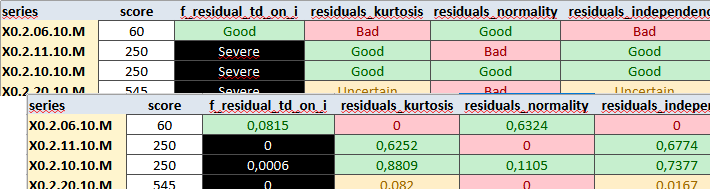
\includegraphics{img/BQ-example.png}

Guided by the quality report, the producer modifies the specifications
to improve seasonal adjustment, generally using the graphical interface.
To generate the final output, particularly the series, they can restart
the \emph{Cruncher}, no longer with the policy=``complete'' option but
using a refresh that re-estimates only the coefficients of the
pre-adjustment model (``policy=regarimaparmeters'') and retains all of
the user's modifications. We provide more details on this point in the
\protect\hyperlink{comp-refresh}{appendices~🔗}.

\begin{Shaded}
\begin{Highlighting}[]
\FunctionTok{library}\NormalTok{(}\StringTok{"rjwsacruncher"}\NormalTok{)}
\FunctionTok{cruncher\_and\_param}\NormalTok{(}
    \AttributeTok{workspace =} \StringTok{"C:/my\_folder/my\_ws.xml"}\NormalTok{,}
    \AttributeTok{rename\_multi\_documents =} \ConstantTok{FALSE}\NormalTok{,}
    \AttributeTok{policy =} \StringTok{"regarimaparameters"}
\NormalTok{)}
\end{Highlighting}
\end{Shaded}

\hypertarget{using-only-r-packages}{%
\section*{Using only R packages}\label{using-only-r-packages}}
\addcontentsline{toc}{section}{Using only R packages}

\markright{Using only R packages}

All of the steps described above can be performed without using a
\emph{workspace} structure and remaining in the R environment.

\hypertarget{estimation-1}{%
\subsection*{Estimation}\label{estimation-1}}
\addcontentsline{toc}{subsection}{Estimation}

In this case, we use the functions
\href{https://rjdverse.github.io/rjd3x13/reference/x13.html}{\VERB|\NormalTok{rjd3x13}\SpecialCharTok{::}\FunctionTok{x13}\NormalTok{()}|
🔗} (or
\href{https://rjdverse.github.io/rjd3tramoseats/reference/tramoseats.html}{\VERB|\NormalTok{rjd3tramoseats}\SpecialCharTok{::}\FunctionTok{tramoseats}\NormalTok{()}|
🔗}) to perform the estimations. Estimation functions work on one TS
object which will require to set up loops or ``lapply'' type functions.

\begin{Shaded}
\begin{Highlighting}[]
\CommentTok{\# for one series }
\NormalTok{mod }\OtherTok{\textless{}{-}} \FunctionTok{x13}\NormalTok{(my\_series, my\_spec)}
\FunctionTok{str}\NormalTok{(mod)}
\end{Highlighting}
\end{Shaded}

\hypertarget{diagnostics-and-specifications}{%
\subsection*{Diagnostics and
specifications}\label{diagnostics-and-specifications}}
\addcontentsline{toc}{subsection}{Diagnostics and specifications}

In R, you can access the same diagnostics as from the GUI and the
\emph{Cruncher} by navigating through the object produced by the
estimation (list of lists), which you can directly organize into a
customized quality report. To take advantage of the existing formatting,
simply rewrite a crunchable \emph{workspace} and regenerate the same
report as in the GUI approach. To remain in one environment, manual
modification of the specifications based on the diagnostics will in this
case be done directly in the R script, as in the example below:

\begin{Shaded}
\begin{Highlighting}[]
\NormalTok{spec0 }\OtherTok{\textless{}{-}}\NormalTok{ rjd3x13}\SpecialCharTok{::}\FunctionTok{x13\_spec}\NormalTok{()}

\NormalTok{spec1\_with\_outliers }\OtherTok{\textless{}{-}}\NormalTok{ rjd3toolkit}\SpecialCharTok{::}\FunctionTok{add\_outlier}\NormalTok{(}
    \AttributeTok{x =}\NormalTok{ spec0,}
    \AttributeTok{type =} \FunctionTok{c}\NormalTok{(}\StringTok{"AO"}\NormalTok{, }\StringTok{"AO"}\NormalTok{, }\StringTok{"LS"}\NormalTok{),}
    \AttributeTok{date =} \FunctionTok{c}\NormalTok{(}\StringTok{"2020{-}02{-}01"}\NormalTok{, }\StringTok{"2020{-}03{-}01"}\NormalTok{, }\StringTok{"2014{-}08{-}01"}\NormalTok{)}
\NormalTok{)}
\end{Highlighting}
\end{Shaded}

The loop of reading diagnostics and modifying parameters is less fluid,
which encourages the use of the graphical interface approach in cases
requiring intensive manual fine-tuning. To update specifications in R
based on diagnostics, scripts must be modified directly, which is slower
and more prone to error for analysts, especially those unfamiliar with
R. The R-only approach makes storing and versioning specifications more
complex.

The diagnostics used to construct the score presented above can be
obtained directly in R, which allows the selective editing procedure to
be replicated. The code for obtaining this output can be found in the
\protect\hyperlink{ind-bq-r}{appendices~🔗}.

The R approach also eliminates any portability issues, even though
updating the link between a \emph{workspace} and the data is now simple
and reliable.

\hypertarget{perf}{%
\section*{Performance}\label{perf}}
\addcontentsline{toc}{section}{Performance}

\markright{Performance}

We compared the performance of the two approaches. The graph below shows
the computation times for seasonally adjusting a dataset, with outlier
detection and calendar effect estimation with a preselected set of
regressors, using the R packages (v2 and v3) or the cruncher (v2 or v3):


\includegraphics{P2-Build_files/figure-pdf/graph-perf-1.pdf}

For a series number close to one thousand, the estimation with
\texttt{rjdx13} takes less than three minutes, which is still very
reasonable for most users but far behind the \emph{Cruncher}, which
completes the same process in about twenty seconds.

Once the production process is in place, it is recommended to validate
or adjust the settings annually and to adopt an infra-annual production
strategy, generally monthly or quarterly, allowing the seasonally
adjusted data to be updated when new raw data becomes available. This
issue is tackled in the next part.

\bookmarksetup{startatroot}

\hypertarget{part-3-infra-annual-and-annual-campaigns}{%
\chapter*{Part 3: Infra-annual and annual
campaigns}\label{part-3-infra-annual-and-annual-campaigns}}
\addcontentsline{toc}{chapter}{Part 3: Infra-annual and annual
campaigns}

\markboth{Part 3: Infra-annual and annual campaigns}{Part 3:
Infra-annual and annual campaigns}

\hypertarget{camp-infra}{%
\subsection*{Infra-annual campaigns}\label{camp-infra}}
\addcontentsline{toc}{subsection}{Infra-annual campaigns}

The objective of an infra-annual campaign is to quickly produce an
updated SA series when a new raw data point is available and the recent
past of the raw series may be revised. The seasonally adjusted series
has two sources of revision: the raw data and changes to the final
seasonal factor estimation models. The seasonal adjustment guidelines
recommend minimizing these so-called technical revisions (see Chapter
6). A common method for achieving this objective is to use the predicted
seasonal factors, including the predicted calendar effect, calculated
during the last annual campaign. However, JDemetra+ also offers a
continuum of refresh methods that allow to gradually loosen the
constraints on the pre-adjustment and control the revisions of the
linearized series before the decomposition step, which will be
completely redone. All of these refresh policies are presented in the
\href{https://doc.jdemetra.org/a-rev-policies}{documentation~🔗}, among
which the ``lastoutliers'' option is particularly recommended. In this
case, we allow ourselves to re-identify the outliers over the last year.
Manual fine-tuning in the infra-annual context will focus on revisions
and therefore outliers, avoiding too many parameter changes. This
refresh is possible from the graphical interface, with the
\emph{Cruncher} by specifying the ``policy'' argument of the
\href{https://aqlt.github.io/rjwsacruncher/reference/cruncher_and_param.html}{\VERB|\NormalTok{rjwsacruncher}\SpecialCharTok{::}\FunctionTok{cruncher\_and\_param}\NormalTok{()}|~🔗}
function but also directly in R with the functions
\VERB|\NormalTok{rjd3x13}\SpecialCharTok{::}\FunctionTok{x13\_refresh}\NormalTok{()}|
or
\VERB|\NormalTok{rjd3tramoseats}\SpecialCharTok{::}\FunctionTok{tramoseats\_refresh}\NormalTok{()}|.

For infra-annual estimation with the \emph{Cruncher}, the following R
code can be used:

\begin{Shaded}
\begin{Highlighting}[]
\FunctionTok{library}\NormalTok{(}\StringTok{"rjwsacruncher"}\NormalTok{)}
\FunctionTok{cruncher\_and\_param}\NormalTok{(}
    \AttributeTok{workspace =} \StringTok{"C:/my\_folder/my\_ws.xml"}\NormalTok{,}
    \AttributeTok{rename\_multi\_documents =} \ConstantTok{FALSE}\NormalTok{,}
    \AttributeTok{policy =} \StringTok{"lastoutliers"}
\NormalTok{)}
\end{Highlighting}
\end{Shaded}

Table 4: Implementation of a refresh policy

\begin{longtable}[]{@{}
  >{\raggedright\arraybackslash}p{(\columnwidth - 2\tabcolsep) * \real{0.5000}}
  >{\raggedright\arraybackslash}p{(\columnwidth - 2\tabcolsep) * \real{0.5000}}@{}}
\toprule\noalign{}
\begin{minipage}[b]{\linewidth}\raggedright
Data type
\end{minipage} & \begin{minipage}[b]{\linewidth}\raggedright
Tools
\end{minipage} \\
\midrule\noalign{}
\endhead
\bottomrule\noalign{}
\endlastfoot
Workspace & - GUI
\href{https://doc.jdemetra.org/a-rev-policies\#implementation-in-gui}{(Drop-down
menus)}\protect\hyperlink{refresh-R}{🔗} \\
& -
\href{https://aqlt.github.io/rjwsacruncher/reference/cruncher_and_param.html}{\VERB|\NormalTok{rjwsacruncher}\SpecialCharTok{::}\FunctionTok{cruncher\_and\_param}\NormalTok{(..., }\AttributeTok{policy=}\NormalTok{ ,)}|~🔗} \\
& -
\href{https://rjdverse.github.io/rjd3workspace/reference/refresh.html}{\VERB|\NormalTok{rjd3workspace}\SpecialCharTok{::}\FunctionTok{jws\_refresh}\NormalTok{()}|~🔗} \\
TS objects in R & -
\href{https://rjdverse.github.io/rjd3x13/reference/refresh.html}{\VERB|\NormalTok{rjd3x13}\SpecialCharTok{::}\FunctionTok{x13\_refresh}\NormalTok{()}|~🔗} \\
& -
\href{https://rjdverse.github.io/rjd3tramoseats/reference/refresh.html}{\VERB|\NormalTok{rjd3tramoseats}\SpecialCharTok{::}\FunctionTok{tramoseats\_refresh}\NormalTok{()}|~🔗} \\
\end{longtable}

The use of forecast seasonal coefficients (\(S\_{f}\)) simply requires
exporting them at the end of the installation process, then at the end
of each annual campaign, in order to perform the calculation:
\(Y_{sa}=Y_{raw}-S_{f}\) or \(Y_{sa}=Y_{raw} / S_{f}\), in the case of a
multiplicative model. To potentially take into account a revision of the
recent past of the raw series, exporting past coefficients is also
useful. The series of forecast coefficients can be generated by the
\emph{Cruncher} by specifying it in the options, as shown below

\begin{Shaded}
\begin{Highlighting}[]
\FunctionTok{options}\NormalTok{(}\AttributeTok{default\_tsmatrix\_series =} \FunctionTok{c}\NormalTok{(}\StringTok{"sa"}\NormalTok{, }\StringTok{"sa\_f"}\NormalTok{, }\StringTok{"s"}\NormalTok{, }\StringTok{"s\_f"}\NormalTok{))}
\end{Highlighting}
\end{Shaded}

or in R by defining a user-defined output as shown below

\begin{Shaded}
\begin{Highlighting}[]
\NormalTok{mod }\OtherTok{\textless{}{-}} \FunctionTok{x13}\NormalTok{(y, }\AttributeTok{userdefined =} \FunctionTok{c}\NormalTok{(}\StringTok{"s"}\NormalTok{, }\StringTok{"s\_f"}\NormalTok{))}
\FunctionTok{str}\NormalTok{(mod}\SpecialCharTok{$}\NormalTok{user\_defined)}
\end{Highlighting}
\end{Shaded}

\hypertarget{camp-an}{%
\subsection*{Annual campaigns}\label{camp-an}}
\addcontentsline{toc}{subsection}{Annual campaigns}

An annual campaign consists of updating seasonal coefficient estimation
models to verify that the parameters used do indeed produce seasonally
adjusted series with the required properties (absence of residual
seasonality, absence of residual calendar effects, etc.).

This update can be done by comparing the current or reference models
used up to the time of the campaign with an automatic estimate. In most
cases, the automatic estimation will be constrained by past parameters
such as the selection of calendar regressors or certain pre-specified
outliers, particularly those from the COVID period. For ease of
comparison, it may be useful to calculate the quality report scores
described in Part 2 for the ``reference'' or ``current''
\emph{workspace} and the ``automatic'' \emph{workspace}. A lower score
for the automatic estimate means that this is preferable, and a new
\emph{workspace} (``working'') can then be created by merging the
``current'' and ``automatic'' \emph{workspaces}, as detailed in the
\protect\hyperlink{fusion-ws}{appendices~🔗}.

This approach requires working on comparable raw series. If these have
undergone significant revisions (re-basing, change of source, etc.), we
return to an approach similar to the installation of a new process.

Main steps:

\begin{itemize}
\item
  Update the reference \emph{workspace} (``ref'') using the new raw data
  and statistical parameters from the previous annual campaign, possibly
  modified by the same strategy as a sub-annual campaign (e.g.,
  ``lastoutliers'').
\item
  Automatic estimation (``auto'') on the new raw data, probably
  maintaining certain parameters (set of calendar regressors, some or
  all of the outliers ``pre-specified'' by the user, etc.)
\item
  calculation of scores for the two \emph{workspaces} ``ref'' and
  ``auto''
\item
  merging of the ``auto'' and ``ref'' \emph{workspaces} into a new
  `working' \emph{workspace} according to the score value of each series
\item
  editing of a quality report on the ``working'' \emph{workspace}
\item
  Manual review with selective editing, as in the installation phase
\item
  Generation of the final output with the \emph{Cruncher}, as in the
  installation phase
\end{itemize}

If forecast coefficients are used during infra-annual campaigns, the
\emph{workspace} from the previous annual campaign can be updated with a
policy ``last outliers'' to return to the case described above.

Details on how the data is organized and code snippets are provided in
the
\href{https://inseefr.github.io/rjd3production/articles/process.html}{vignette
\{rjd3production\} package 🔗}.

\hypertarget{numerical-impact-of-a-change-in-parameters}{%
\subsection*{Numerical impact of a change in
parameters}\label{numerical-impact-of-a-change-in-parameters}}
\addcontentsline{toc}{subsection}{Numerical impact of a change in
parameters}

In light of the (bad) diagnostics, identified in particular through the
quality report, the producer can intervene to modify the parameters and
improve the statistical quality of the adjustment. For example, they can
modify a set of calendar regressors and eliminate the residual calendar
effects that they had previously observed. Beyond improving statistical
test results, it is often useful to visualize the numerical impact of a
parameter change or re-estimation, which allows revisions to be
quantified and visualized, but also certain settings to be validated,
particularly the choice of outliers based on ``expert knowledge.''
Exporting the series produced is one solution, but if you want to make
these comparisons before you have finished working on a
\emph{workspace}, you can use the
\href{https://inseefr.github.io/rjd3production/reference/compare.html}{\VERB|\FunctionTok{compare}\NormalTok{()}|~🔗}
function from the rjd3production package, which avoids generating
intermediate outputs. This allows you to read the series directly in two
or more \emph{workspaces}, each corresponding to a version of the
parameters or a state of the estimate, as shown in the following code:

\begin{Shaded}
\begin{Highlighting}[]
\NormalTok{df }\OtherTok{\textless{}{-}} \FunctionTok{compare}\NormalTok{(path\_ws\_ref, path\_ws\_work)}
\FunctionTok{run\_app}\NormalTok{(df)}
\end{Highlighting}
\end{Shaded}

The function launches a shiny application that provides a graphical
comparison, below is the final trend (d12), and the ability to download
the series values to analyse the revisions.

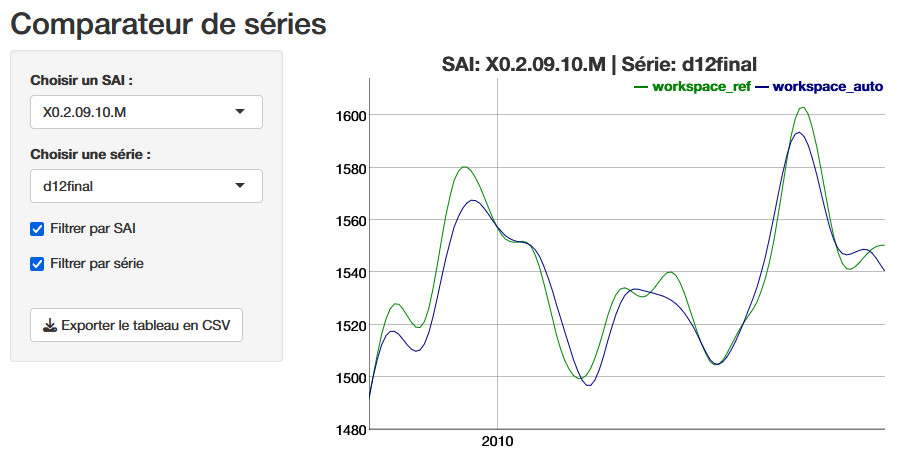
\includegraphics{img/shiny-app.png}

\hypertarget{conclusion}{%
\section*{Conclusion}\label{conclusion}}
\addcontentsline{toc}{section}{Conclusion}

\markright{Conclusion}

Ensuring the statistical quality of seasonally adjusted series requires
the implementation of a production process that, in light of
diagnostics, allows for easy and large-scale customization of estimation
parameters. The use of the open-source software JDemetra+ and its R
tools makes it possible to achieve this goal by offering various
automation options while providing access to detailed manual fine
tuning. We have seen that the decision to integrate the graphical user
interface into a production process is fundamental to the organization
of data. The main reasons for this should be the use of manual
fine-tuning and performance. However, an organization based solely on R
does not exclude ad hoc use of the GUI or \emph{Cruncher}. The
organization of operations and the use of tools as described in this
article are, of course, only suggestions, which we hope will provide
practical answers to the many producers of SA series who wish to use
JDemetra+.

In order to communicate with their users, they often need reporting
tools that break down the effects of seasonal adjustment on changes in a
given series, in particular to highlight the various contributions to
revisions. Such tools are often \emph{in-house}, but there are packages
or plug-ins linked to JDemetra+, often still in version 2, that allow to
display this type of information. It would be interesting to follow up
on this article by offering a review of open-source reporting tools and
making available an R package that allows users to take full advantage
of version 3 of JDemetra+.

\pagebreak

\bookmarksetup{startatroot}

\hypertarget{appendices}{%
\chapter*{Appendices}\label{appendices}}
\addcontentsline{toc}{chapter}{Appendices}

\markboth{Appendices}{Appendices}

\hypertarget{crea-regs}{%
\section*{Calendar effect correction}\label{crea-regs}}
\addcontentsline{toc}{section}{Calendar effect correction}

\markright{Calendar effect correction}

There are two possible procedures for generating calendar regressors:
creating customized regressors as shown below, or using predefined
regressors in JDemetra+, which also requires defining a reference
calendar. Version 3.x of the GUI allows you to automatically {[}select
🔗)(https://doc.jdemetra.org/a-sa-pre-treatment\#calendar-correction)
from the predefined regressor sets, based on statistical tests.

Instead of a simple
\href{https://doc.jdemetra.org/a-calendar-correction\#national-calendar}{national
calendar 🔗}, JDemetra+ allows you to create
\href{https://doc.jdemetra.org/a-calendar-correction\#chained-calendar}{``chained''
🔗} or
\href{https://doc.jdemetra.org/a-calendar-correction\#composite-calendar}{``composite''
🔗} with the GUI or
\href{https://rjdverse.github.io/rjd3toolkit/reference/index.html\#calendars}{rjd3toolkit
🔗}.

\hypertarget{creating-a-reference-calendar}{%
\subsection*{Creating a reference
calendar}\label{creating-a-reference-calendar}}
\addcontentsline{toc}{subsection}{Creating a reference calendar}

To create a French calendar based on French public holidays, you can use
the
\href{https://inseefr.github.io/rjd3production/reference/insee_modelling.html}{\texttt{create\_french\_calendar()}~🔗}
function from the \{rjd3production\} package:

\begin{Shaded}
\begin{Highlighting}[]
\NormalTok{cal\_FR }\OtherTok{\textless{}{-}} \FunctionTok{create\_french\_calendar}\NormalTok{()}
\end{Highlighting}
\end{Shaded}

This function can be adapted to any national calendar.

\hypertarget{generation-of-regressor-sets}{%
\subsection*{Generation of regressor
sets}\label{generation-of-regressor-sets}}
\addcontentsline{toc}{subsection}{Generation of regressor sets}

Using the French calendar, it is possible to generate calendar
regressors based, for example, on the usual groups used by INSEE:

\begin{Shaded}
\begin{Highlighting}[]
\NormalTok{regs }\OtherTok{\textless{}{-}} \FunctionTok{create\_insee\_regressors}\NormalTok{(}\AttributeTok{start =} \FunctionTok{c}\NormalTok{(}\DecValTok{2000}\NormalTok{, }\DecValTok{1}\NormalTok{), }\AttributeTok{frequency =} \DecValTok{12}\NormalTok{, }\AttributeTok{length =} \DecValTok{360}\NormalTok{)}
\NormalTok{sets }\OtherTok{\textless{}{-}} \FunctionTok{create\_insee\_regressors\_sets}\NormalTok{(}\AttributeTok{start =} \FunctionTok{c}\NormalTok{(}\DecValTok{2000}\NormalTok{, }\DecValTok{1}\NormalTok{), }\AttributeTok{frequency =} \DecValTok{12}\NormalTok{, }\AttributeTok{length =} \DecValTok{240}\NormalTok{)}
\FunctionTok{names}\NormalTok{(sets)}
\end{Highlighting}
\end{Shaded}

\begin{verbatim}
 [1] "REG1"    "REG2"    "REG3"    "REG5"    "REG6"    "LY"      "REG1_LY"
 [8] "REG2_LY" "REG3_LY" "REG5_LY" "REG6_LY"
\end{verbatim}

\hypertarget{ind-bq-r}{%
\section*{Quality Report: Diagnostics and R code}\label{ind-bq-r}}
\addcontentsline{toc}{section}{Quality Report: Diagnostics and R code}

\markright{Quality Report: Diagnostics and R code}

Diagnostics selected by default when using
X-13-Arima\footnote{When using Tramo-Seats, this also works, but in this version, the diagnostics specific to X-13-Arima are simply removed and not replaced}
are as follows:

Table A1: Diagnostics

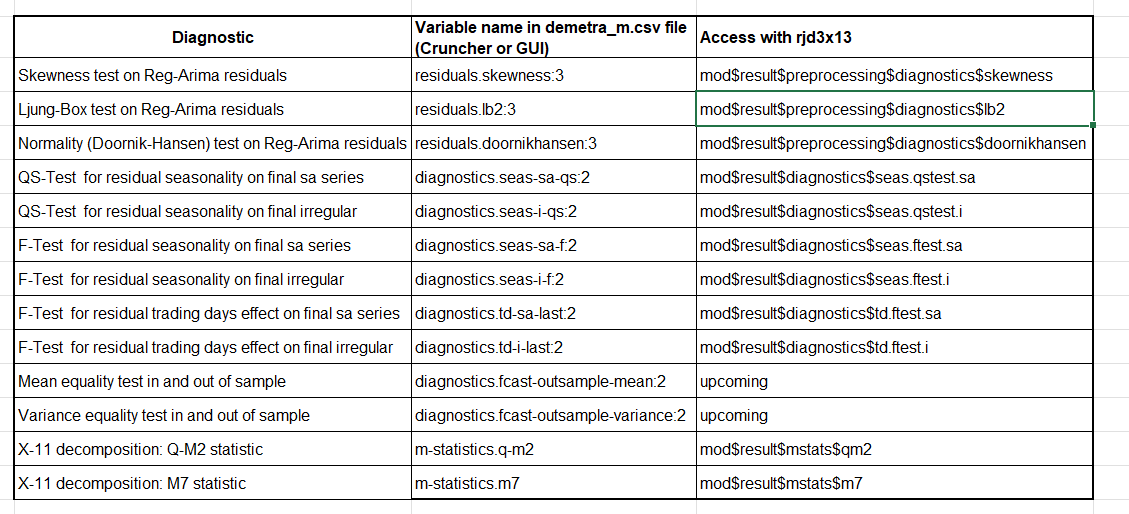
\includegraphics{img/BQ-Output-EN.png}

In R, the diagnostics are extracted from the ``m\_sa'' object containing
all the estimation results and obtained with the code below.

\begin{Shaded}
\begin{Highlighting}[]
\NormalTok{m\_sa }\OtherTok{\textless{}{-}} \FunctionTok{x13}\NormalTok{(my\_series, my\_spec, }\AttributeTok{userdefined =} \FunctionTok{c}\NormalTok{(}\StringTok{"diagnostics.fcast{-}outsample{-}mean"}\NormalTok{,}\StringTok{"diagnostics.fcast{-}outsample{-}variance"}\NormalTok{))}
\FunctionTok{str}\NormalTok{(m\_sa)}
\end{Highlighting}
\end{Shaded}

More information on the tests is available in the
\href{https://doc.jdemetra.org/m-tests}{documentation 🔗}

\hypertarget{eq-score}{%
\subsection*{Score equation}\label{eq-score}}
\addcontentsline{toc}{subsection}{Score equation}

\[
\begin{aligned}
score\_total &= 30 * grade\_qs\_residual\_s\_on\_sa\\
&+ 30 * grade\_f\_residual\_s\_on\_sa\\
&+ 30 * grade\_f\_residual\_td\_on\_sa\\
&+ 20 * grade\_f\_residual\_td\_on\_i\\
&+ 20 * grade\_qs\_residual\_sa\_on\_i\\
&+ 20 * grade\_f\_residual\_sa\_on\_i\\
&+ 15 * grade\_oos\_mean\\
&+ 10 * grade\_oos\_mse\\
&+ 15 * grade\_residuals\_independency\\
&+ 5 * grade\_residuals\_skewness\\
&+ 5 * grade\_residuals\_homoskedasticity\\
&+ 5 * grade\_q\_m2\\
&+ 5 * grade\_m7
\end{aligned}
\]

\hypertarget{annual-campaign-comparison-of-workspaces}{%
\section*{Annual campaign: comparison of
workspaces}\label{annual-campaign-comparison-of-workspaces}}
\addcontentsline{toc}{section}{Annual campaign: comparison of
workspaces}

\markright{Annual campaign: comparison of workspaces}

\hypertarget{merge-ws}{%
\subsection*{Creation of WS\_work}\label{merge-ws}}
\addcontentsline{toc}{subsection}{Creation of WS\_work}

The \textbf{WS\_work} is a merger between \textbf{WS\_ref} and
\textbf{WS\_auto}. A score is calculated for both \emph{workspaces} and,
for each series, the SA-Item is retrieved from the \emph{workspace} with
the lowest score between WS\_auto and WS\_ref.

In an annual campaign process, we will use the
\href{https://rjdverse.github.io/rjd3workspace/reference/transfer_sa_item.html}{\VERB|\FunctionTok{transfer\_sa\_item}\NormalTok{()}|
🔗} function from \{rjd3workspace\} to merge \textbf{WS\_ref} and
\textbf{WS\_auto}.

\begin{Shaded}
\begin{Highlighting}[]
\CommentTok{\# save WS\_ref as initial version of WS\_work}
\NormalTok{WS\_auto }\OtherTok{\textless{}{-}} \FunctionTok{load\_workspace}\NormalTok{(}\AttributeTok{file =} \StringTok{"./WS/WS\_auto.xml"}\NormalTok{)}
\NormalTok{WS\_work }\OtherTok{\textless{}{-}} \FunctionTok{load\_workspace}\NormalTok{(}\AttributeTok{file =} \StringTok{"./WS/WS\_work.xml"}\NormalTok{)}

\NormalTok{sap1\_auto }\OtherTok{\textless{}{-}} \FunctionTok{.jws\_sap}\NormalTok{(}\AttributeTok{jws =}\NormalTok{ WS\_auto, }\AttributeTok{idx =} \DecValTok{1}\NormalTok{)}
\NormalTok{sap1\_work }\OtherTok{\textless{}{-}} \FunctionTok{.jws\_sap}\NormalTok{(}\AttributeTok{jws =}\NormalTok{ WS\_work, }\AttributeTok{idx =} \DecValTok{1}\NormalTok{)}

\CommentTok{\# update ws\_work with sa{-}items from ws auto when necessary }
\FunctionTok{transfer\_series}\NormalTok{(}
    \AttributeTok{jsap\_from =}\NormalTok{ sap1\_auto,}
    \AttributeTok{jsap\_to =}\NormalTok{ sap1\_work,}
    \AttributeTok{selected\_sa\_items =} \FunctionTok{c}\NormalTok{(}\StringTok{"RF0610"}\NormalTok{, }\StringTok{"RF0620"}\NormalTok{)}
\NormalTok{)}

\FunctionTok{save\_workspace}\NormalTok{(}\AttributeTok{jws =}\NormalTok{ WS\_work, }\AttributeTok{file =} \StringTok{"./WS/WS\_work.xml"}\NormalTok{)}
\end{Highlighting}
\end{Shaded}

\hypertarget{comp-specs}{%
\section*{Additional information on specifications}\label{comp-specs}}
\addcontentsline{toc}{section}{Additional information on specifications}

\markright{Additional information on specifications}

\hypertarget{modification}{%
\subsection*{Modification}\label{modification}}
\addcontentsline{toc}{subsection}{Modification}

\begin{itemize}
\tightlist
\item
  \texttt{Reference\ Specification}
\end{itemize}

Modification in the GUI:


\includegraphics[width=0.9\textwidth,height=0.6\textheight]{../../img/DT_modif_ref_spec.png}

Using this same menu, you can apply the
\texttt{Reference\ Specification} or the \texttt{Result\ Specification}
to a series.

In the \texttt{rjd3workspace} package:

\begin{Shaded}
\begin{Highlighting}[]
\FunctionTok{library}\NormalTok{(}\StringTok{"rjd3workspace"}\NormalTok{)}
\FunctionTok{set\_reference\_specification}\NormalTok{(jsap, 1L, new\_reference\_spec)}
\end{Highlighting}
\end{Shaded}

\begin{itemize}
\tightlist
\item
  \texttt{Estimation\ Specification}
\end{itemize}

Modification in GUI, use the \texttt{Specification} button on the
right-hand side:


\includegraphics[width=0.9\textwidth,height=0.6\textheight]{../../img/DT_modif_est_spec.png}

In the \texttt{rjd3workspace} package,
\texttt{Estimation\ Specification} is simply referred to as
\texttt{Specification}:

\begin{Shaded}
\begin{Highlighting}[]
\FunctionTok{library}\NormalTok{(}\StringTok{"rjd3workspace"}\NormalTok{)}
\FunctionTok{set\_specification}\NormalTok{(jsap, 1L, new\_estimation\_spec)}
\end{Highlighting}
\end{Shaded}

\begin{itemize}
\tightlist
\item
  \texttt{Result\ Specification}
\end{itemize}

Estimation result can be applied as indicated below.

\begin{Shaded}
\begin{Highlighting}[]
\FunctionTok{library}\NormalTok{(}\StringTok{"rjd3workspace"}\NormalTok{)}

\FunctionTok{jws\_compute}\NormalTok{(jws)}
\FunctionTok{read\_workspace}\NormalTok{(jws, }\AttributeTok{compute =} \ConstantTok{TRUE}\NormalTok{)}
\FunctionTok{read\_sap}\NormalTok{(jsap)}
\FunctionTok{read\_sai}\NormalTok{(jsai)}
\end{Highlighting}
\end{Shaded}

\hypertarget{comp-refresh}{%
\subsection*{Refresh policy behavior}\label{comp-refresh}}
\addcontentsline{toc}{subsection}{Refresh policy behavior}

A refresh policy is designed to remove all or some of the constraints
from the \texttt{Estimation\ Specification} and revert to the
\texttt{Reference\ Specification}.

\begin{itemize}
\item
  The ``concurrent'' policy reverts to the
  \texttt{Reference\ Specification} by clearing user-defined parameters
  not written in the reference spec (changes made via the specification
  window on the right hand side are discarded). In particular, it clears
  the outliers pre-specified in the \texttt{Estimation\ Specification};
  all outliers will be re-identified
\item
  The ``lastoutliers'' policy clears the outliers pre-specified in the
  \texttt{Estimation\ Specification} for the last year (or other defined
  span); re-identification will be performed for this period.
\end{itemize}

This allows the user to distinguish between permanent settings
(\texttt{Reference\ Specification}) and temporary settings
(\texttt{Estimation\ Specification}).

\hypertarget{example}{%
\subsection*{Example}\label{example}}
\addcontentsline{toc}{subsection}{Example}

Here is a common procedure for updating data in the case of an
intra-annual campaign, with output generation using \emph{Cruncher}.
Note: You must save the \emph{workspace} before performing a ``refresh''
(via the GUI or \emph{Cruncher}).

\begin{itemize}
\item
  New raw data is available (new data points and revisions to recent
  history).
\item
  Use a ``refresh last outliers'' to benefit from automatic detection
  for the last year
\item
  Check the results and revisions; for certain important series, you may
  want to review the automatic detection
\item
  We open the graphical interface and modify the
  \texttt{Estimation\ Specification} for a series via the window on the
  right by adding an outlier (\(Out_1\)) in the last year
\item
  We apply and save these changes in the GUI
\item
  We must regenerate an output with the \emph{Cruncher} (export of final
  series)
\item
  If the \emph{Cruncher} uses ``policy=lastoutliers'' again: it reverts
  to the \texttt{Reference\ Specification} for the last year, and
  \(Out_1\) is lost
\item
  If you want to keep \(Out_1\), use the option policy =
  ``arimaparameters''; the identification remains unchanged, only the
  coefficients are re-estimated
\item
  To keep \(Out_1\) and re-identify using ``lastoutliers'' again, you
  must include \(Out_1\) in the \texttt{Reference\ Specification}.
\end{itemize}

\hypertarget{spec-v2-v3}{%
\subsection*{Differences between version 2 and version
3}\label{spec-v2-v3}}
\addcontentsline{toc}{subsection}{Differences between version 2 and
version 3}

In JDemetra+ version 2.x, there was no
\texttt{Estimation\ Specification}. The settings set by the user were
therefore necessarily saved in the \texttt{Reference\ Specification} and
hence never deleted by a refresh policy.

\emph{workspaces} created in version 2 can be opened in version 3, but
it will no longer be possible to return to version 2.

Copying specifications when a version 2 \emph{workspace} is opened in
version 3:

\begin{itemize}
\item
  \texttt{Reference\ Specification} is copied in
  \texttt{Reference\ Specification} and in
  \texttt{Estimation\ Specification}
\item
  \texttt{Result\ Specification} is copied in
  \texttt{Result\ Specification}
\end{itemize}

\hypertarget{data-structures-1}{%
\section*{Data structures}\label{data-structures-1}}
\addcontentsline{toc}{section}{Data structures}

\markright{Data structures}

\emph{workspaces} are organized into SA-Processing and SA-Item.

\hypertarget{sec-concept-sap}{%
\subsection*{SA-Processing}\label{sec-concept-sap}}
\addcontentsline{toc}{subsection}{SA-Processing}

An SA-Processing (SAP) is represented by an \texttt{.xml} file. It
contains SA-Items and user-defined reference specifications.

\hypertarget{sec-concept-sai}{%
\subsection*{SA-Item}\label{sec-concept-sai}}
\addcontentsline{toc}{subsection}{SA-Item}

An SA-Item contains information about a given series:

\begin{itemize}
\item
  raw data
\item
  specifications (\texttt{resultSpecification},
  \texttt{estimationSpecification})
\item
  metadata
\end{itemize}

\hypertarget{sec-concept-metadata}{%
\subsection*{Metadata}\label{sec-concept-metadata}}
\addcontentsline{toc}{subsection}{Metadata}

The metadata (see the tag in the \texttt{.xml} file corresponding to
SA-Processing) contains:

\begin{itemize}
\item
  the type of source of the raw data
\item
  the ``id'' of the file containing the raw data (path and parameters)
  that will be used to refresh the estimate
\item
  any comments on the series (generally used to justify a choice of
  parameters)
\end{itemize}

\hypertarget{sec-concept-modelling-context}{%
\subsection*{Modelling context}\label{sec-concept-modelling-context}}
\addcontentsline{toc}{subsection}{Modelling context}

The modelling context contains the calendars, variables, and external
regressors needed for the estimates made in the \emph{workspace}.

\hypertarget{mig-to-jd}{%
\section*{Migration to JDemetra+}\label{mig-to-jd}}
\addcontentsline{toc}{section}{Migration to JDemetra+}

\markright{Migration to JDemetra+}

It is possible to convert X-13 specifications used in the US Census
Bureau's X-13-Arima-Seats software into JDemetra+ X13-Arima
specifications.

This operation is performed using the graphical interface with the
\href{https://github.com/bbkrd/SpecParser}{SpecParser~🔗} plug-in, which
can only be used in version 2. The \emph{workspace} containing these
specifications can be opened in version 3. The plug-in documentation can
be found \href{https://bbkrd.github.io/pages/specparser/}{here~🔗} and
all the migration steps are described
\href{https://bbkrd.github.io/pages/specparser/}{here~🔗} in the
JDemetra+ documentation.

\bookmarksetup{startatroot}

\hypertarget{references}{%
\chapter*{References}\label{references}}
\addcontentsline{toc}{chapter}{References}

\markboth{References}{References}

\hypertarget{refs}{}
\begin{CSLReferences}{1}{0}
\leavevmode\vadjust pre{\hypertarget{ref-attal2012regresseurs}{}}%
Attal Toubert, Ketty. 2012. {``R{é}gresseurs Pour Effets de Calendrier:
Comment Les Construire, Comment Les Choisir.''} \emph{XI{è}mes
Journ{é}es de M{é}thodologie Statistique de l'Insee}.

\leavevmode\vadjust pre{\hypertarget{ref-bell1984issues}{}}%
Bell, William R, and Steven C Hillmer. 1984. {``Issues Involved with the
Seasonal Adjustment of Economic Time Series.''} \emph{Journal of
Business \& Economic Statistics} 2 (4): 291--320.

\leavevmode\vadjust pre{\hypertarget{ref-eurostat2024guidelines}{}}%
Eurostat. 2024. {``ESS Guidelines on Seasonal Adjustment.''} Eurostat
Methodologies; Working Papers, European Commission.
\href{https://doi.org/10.2785/705102\%20}{https://doi.org/10.2785/705102
}.

\leavevmode\vadjust pre{\hypertarget{ref-gomez1996programs}{}}%
Gomez, Victor, and Agustin Maravall. 1996. {``Programs TRAMO (Time
Series Regression with Arima Noise, Missing Observations, and Outliers)
and SEATS (Signal Extraction in Arima Time Series). Instructions for the
User.''} \emph{Documento de Trabajo} 9628: 56.

\leavevmode\vadjust pre{\hypertarget{ref-grudkowska2013advanced}{}}%
Grudkowska, Sylwia, Dario Buono, Jean Palate, and Wojciech Ciebiera.
2013. {``Advanced Tools for Time Series Analysis and Seasonal Adjustment
in the New Jdemetra+.''} \emph{JSM Proceedings Paper}.

\leavevmode\vadjust pre{\hypertarget{ref-ch22HBSA}{}}%
Kirchner, and alli. 2018. {``Quality Measures and Reporting for Seasonal
Adjustment.''} \emph{Handbook on Seasonal Adjustment}.
\href{https://ec.europa.eu/eurostat/web/products-manuals-and-guidelines/-/KS-GQ-18-001}{ec.europa.eu/eurostat/web/products-manuals-and-guidelines/-/KS-GQ-18-001}.

\leavevmode\vadjust pre{\hypertarget{ref-JD_doc}{}}%
Smyk, and alli. 2026. {``Online JD+ Documentation.''} 2026.
\url{https://jdemetra-new-documentation.netlify.app/}.

\leavevmode\vadjust pre{\hypertarget{ref-census}{}}%
US-Census-Bureau. 2015. {``The x-13ARIMA-Seats Seasonal Adjustment
Program.''} 2015. \url{https://www.census.gov/srd/www/x13as}.

\leavevmode\vadjust pre{\hypertarget{ref-webel2024seasonal}{}}%
Webel, Karsten, and Anna Smyk. 2024. {``Seasonal Adjustment of
Infra-Monthly Time Series with JDemetra+.''} \emph{Journal of Official
Statistics} 40 (4): 783--828.

\end{CSLReferences}



\end{document}
